%------------------------------------------------------------------------------------
\newpage
\section{Практическая часть}

На рис.~(\ref{fig:ber_ofdm}) показаны кривые зависимости вероятности битовой ошибки (BER)
от отношения сигнал/шум (SNR) для OFDM сигнала с модуляцией ФМ-16 и количеством поднесущих
$N = 2048$.

%------------------------------------------------------------------------------------
% Figure
%------------------------------------------------------------------------------------
\begin{figure}[h]
    \centering
    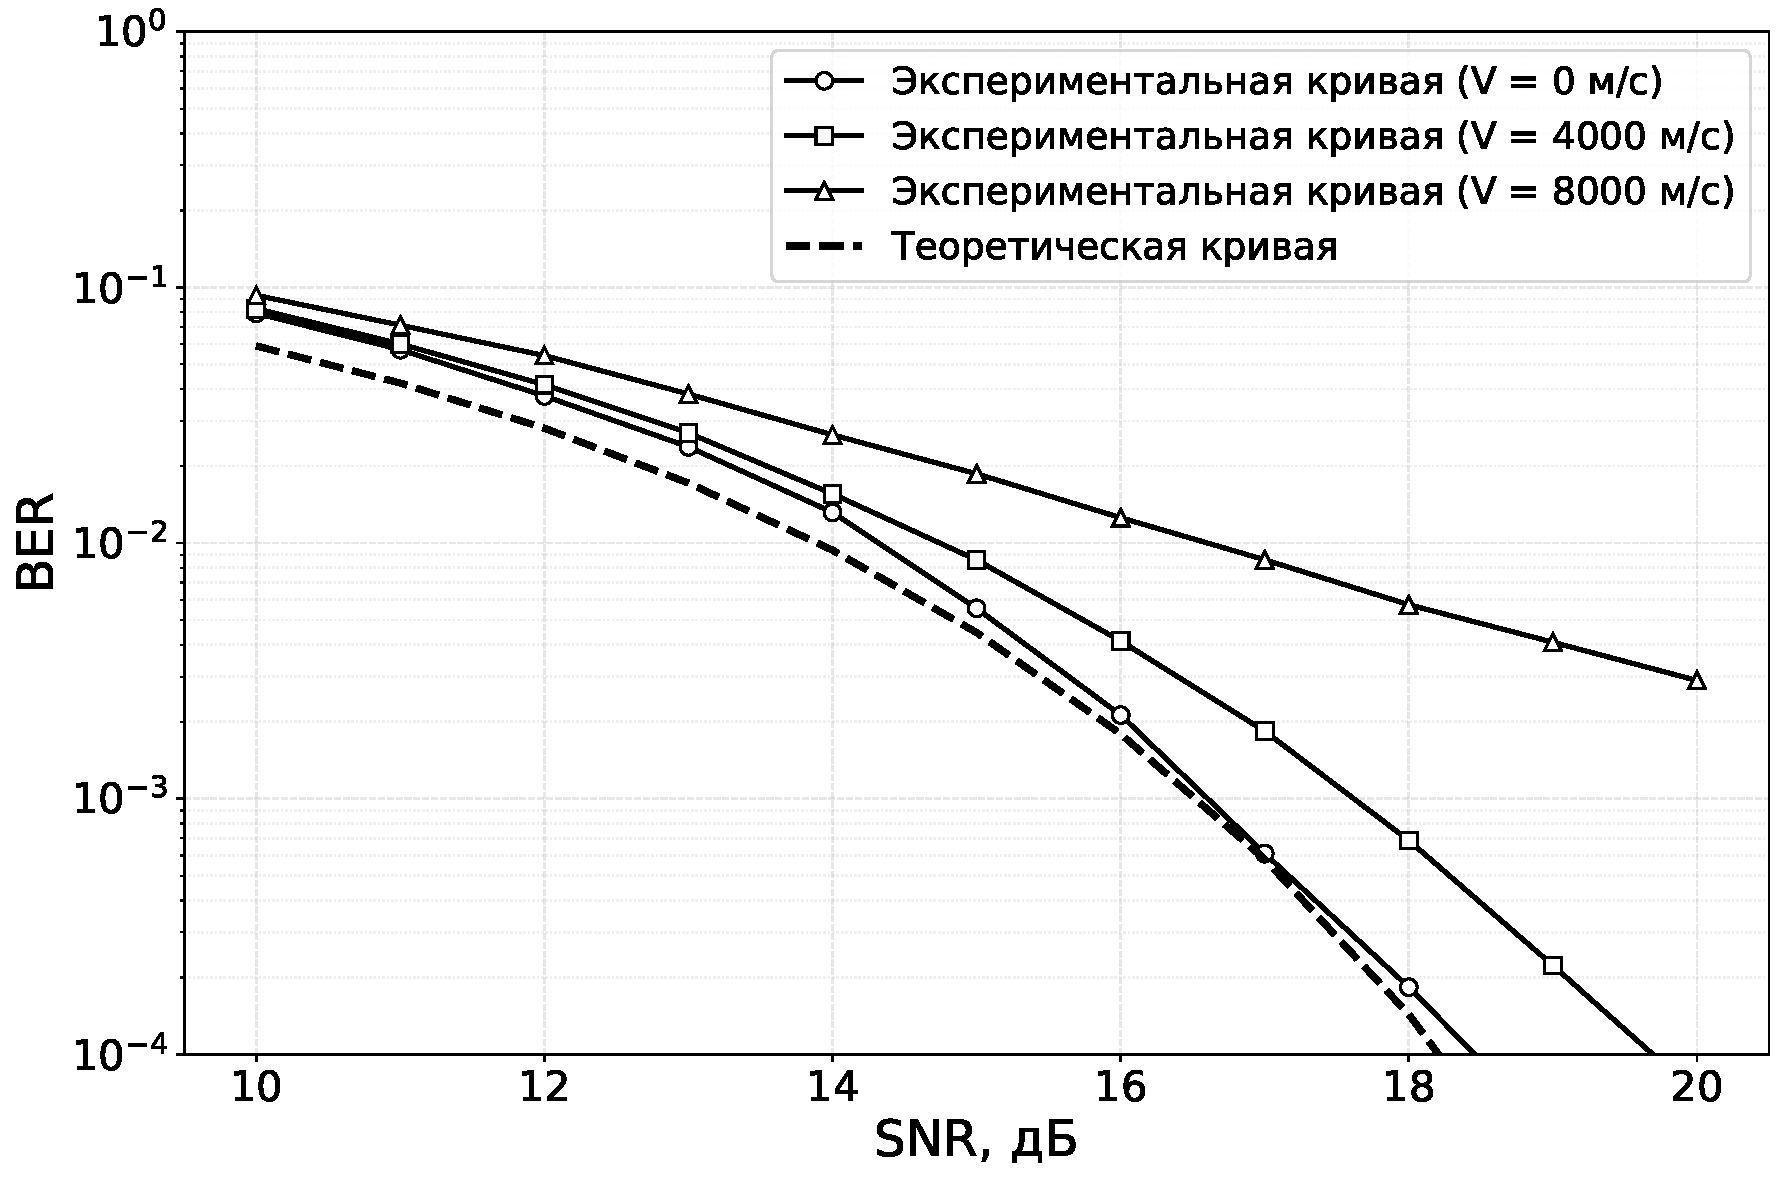
\includegraphics[width=1\textwidth]{images/2_ber_ofdm_qam_16.pdf}
    \caption{Зависимость вероятности биторой ошибки (BER) от отношения сигнал/шум (SNR)
             для различных значений модуля относительной скорости }
    \label{fig:ber_ofdm}
\end{figure}
\FloatBarrier
%------------------------------------------------------------------------------------

На рис.~(\ref{fig:ber_ofdm_subc}) показаны кривые зависимости вероятности битовой ошибки (BER)
от отношения сигнал/шум (SNR) для OFDM сигнала с модуляцией ФМ-16 и модулем относительной скорости 
$V = 8000 м/c$.

%------------------------------------------------------------------------------------
% Figure
%------------------------------------------------------------------------------------
\begin{figure}[h]
    \centering
    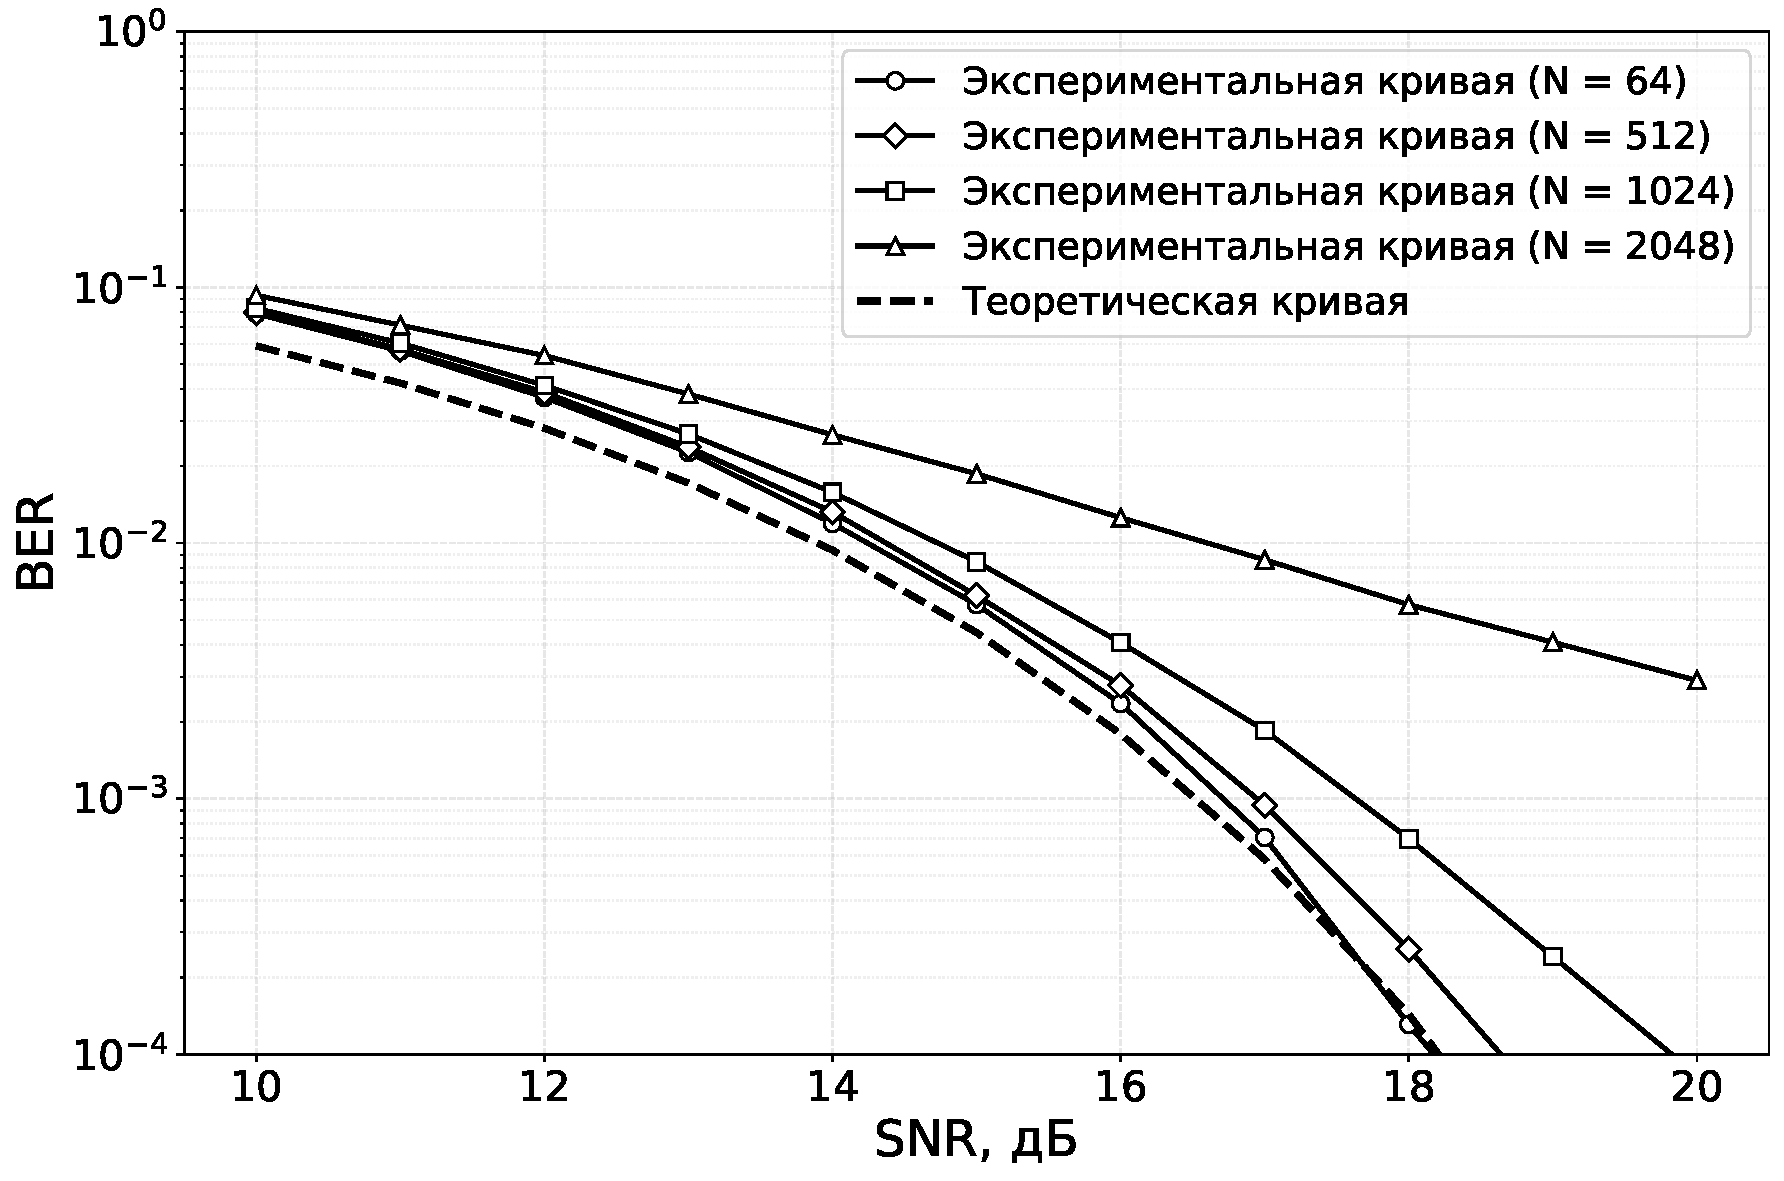
\includegraphics[width=1\textwidth]{images/2_ber_ofdm_qam_16_subc.pdf}
    \caption{Зависимость вероятности биторой ошибки (BER) от отношения сигнал/шум (SNR)
             для различных значений количества поднесущих}
    \label{fig:ber_ofdm_subc}
\end{figure}
\FloatBarrier
%------------------------------------------------------------------------------------